%
% Another appendix chapter
\chapter{Toward Application: Walking}\label{chap:walking}
The control strategy for a static, standing case presented in the previous chapter is two-dimensional. If the robot is walking, the motion of the \ac{CoM} relative to the ground reference point might not be \textit{aligned} with the direction of the error. In this chapter, the bang-bang control law of Chapter \ref{chap:standing} is extended for the use in \ac{3D}.
% Experimental Setup
\section{Experimental Setup}
With the same motivation as in the previous chapter of applying a maximum acceleration possible in a worst-case scenario, a bang-bang control law can be used. In this section, to determine \textit{when} to turn the bang-bang controller on in \ac{3D},  tests are conducted preliminary to developing a controller. 

In this test, a push is applied in the beginning of the \ac{SS} while the robot is walking. The stepping parameters used for the test situation are given in Table \ref{tab:stepping}, which are the default stepping parameters during testing in simulation. In \figref{fig:valwalkingtest}, the test setup in simulation is shown. The limited foothold options display that footstep location adjustment is not available as a balance strategy. In \figref{fig:3foot}, the \ac{ICP} reference trajectory and the measured \ac{CoM} trajectory, without application of a push are made visible. 
\begin{table}[ht]
\caption{Stepping Parameters} % title of Table
\centering % used for centering table
\begin{tabular}{c c c } % centered columns (4 columns)
\hline\hline %inserts double horizontal lines
Parameter & Value & Unit \\
%heading
\hline % inserts single horizontal line
Step Legth & 0.5 &  [m]\\
Step Width & 0.25 & [m]\\
\acs{SS} Time & 0.6 & [s]\\
\acs{DS} Time & 0.15 & [s]\\
%[1ex] % [1ex] adds vertical space
\hline %inserts single line
\end{tabular}
\label{tab:stepping} % is used to refer this table in the text
\end{table}
\begin{figure}[h]
\centering
  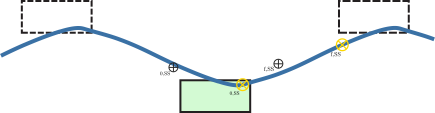
\includegraphics[width=.8\linewidth]{STYLESTUFF/ICPplan3StepComICPrSS.png}
   \caption{Trajectories during \ac{SS} in the horizontal plane (gray dotted lines). The gray area is the current footstep position.}
    \label{fig:3foot}
\end{figure}
\begin{figure}[h]
\centering
  \includegraphics[width=.8\linewidth]{STYLESTUFF/valwalkingtest.png}
   \caption{.}
    \label{fig:valwalkingtest}
\end{figure}
\subsection{Preliminary Observations}
%Preliminary observations
The following properties are observed, when applying pushes in different direction in the start of \ac{SS}.
\begin{itemize}
	\item The direction of the \ac{ICP} error stays often approximately the same until transition to \ac{DS}.
	\item If the \ac{ICP} error is directed in the sagittal plane, the desired \ac{CMP} often remains somewhat in the same location.
	\item If the \ac{ICP} error is directed  in the coronal plane, the desired \ac{CMP} slides from back to the forth of the foot.
	\item The configuration and velocity near transition to \ac{DS} affects the robots ability to put its swing leg down at the desired time. 
\end{itemize}

In \ac{3D}, the problem is that the \textit{virtual leg} between $\rcopd$ and the \ac{CoM} $\cxy$ might not be \textit{aligned} with the \ac{ICP} error $\icpe$. Furthermore, the $\textit{effective horizontal distance}$ between $\rcopd$ and $\cxy$ might be very small. During stance, this effective horizontal distance is always approximately the same value: the \ac{CoM} is in the center of the polygon and $\rcopd$ is on the polygon edge in a worst-case scenario. During walking however, the effective horizontal distance changes and in some cases height variations are not contributing to balance control. This can also be derived from the \ac{VHIP} dynamical model from Equation \ref{eq:dynamicscaronstyle}. Vertical \ac{CoM} motion at a shorter horizontal distance between the virtual point foot and the \ac{CoM} affects the horizontal dynamics relatively less.

In Figure \ref{fig:phiViz}, the following two variable are explained by an \ac{ICP} error in the start of \ac{SS}:
\begin{itemize}
	\item $\phi$: the alignment angle between the virtual leg between $\rcopd$ and $\cxy$ and the \ac{ICP} error $\icpe$;
	\item $\delta$: the effective distance between $\rcopd$ and $\cxy$. The is the distance between the two points in the direction of the \ac{ICP} error $\icpe$.
\end{itemize}
In Figure \ref{fig:phiViza}, $\icpe$ is positive, resulting from a frontal push. This results in a $\rcopd$ in the rear side of the support foot polygon. The distance $\delta$ is small, and $\phi$ is fairly misaligned. This is a relatively bad condition to use vertical motion for balance. However, the alignment angle in the end of \ac{SS}, $\phi_f$, is relatively good. In Figure \ref{fig:phiVizb}, $\icpe$ is negative, resulting from a bush in the back. The distance $\delta$ is relatively large and $\phi$ is more aligned.  Also, there is room left for control by $\rcopd$ in the coronal plane. This is a relatively good condition to use vertical motion. In Figure \ref{fig:phiVizc}, $\phi=0$ and $\delta$ is large, a good condition for vertical motion. In Figure \ref{fig:phiVizd}, $\delta=0$ and $\phi=\frac{1}{2}\pi$, a bad condition for vertical motion. In Figure \ref{fig:phiVize}, $\phi$ plays a less important roll, as $\rcmpd$ is expected to move from the back to the front of the foot. This allows for control by $\rcopd$ in the sagittal plane. The distance $\delta$ plays a more important role, which is of an intermediate size. In Figure \ref{fig:phiVizf}, the same case holds for the angle $\phi$ as in the previous figure, but the distance $\delta$ is smaller this time.  
\begin{figure}[h]
\centering
  \begin{subfigure}{0.4\textwidth}
  \centering
  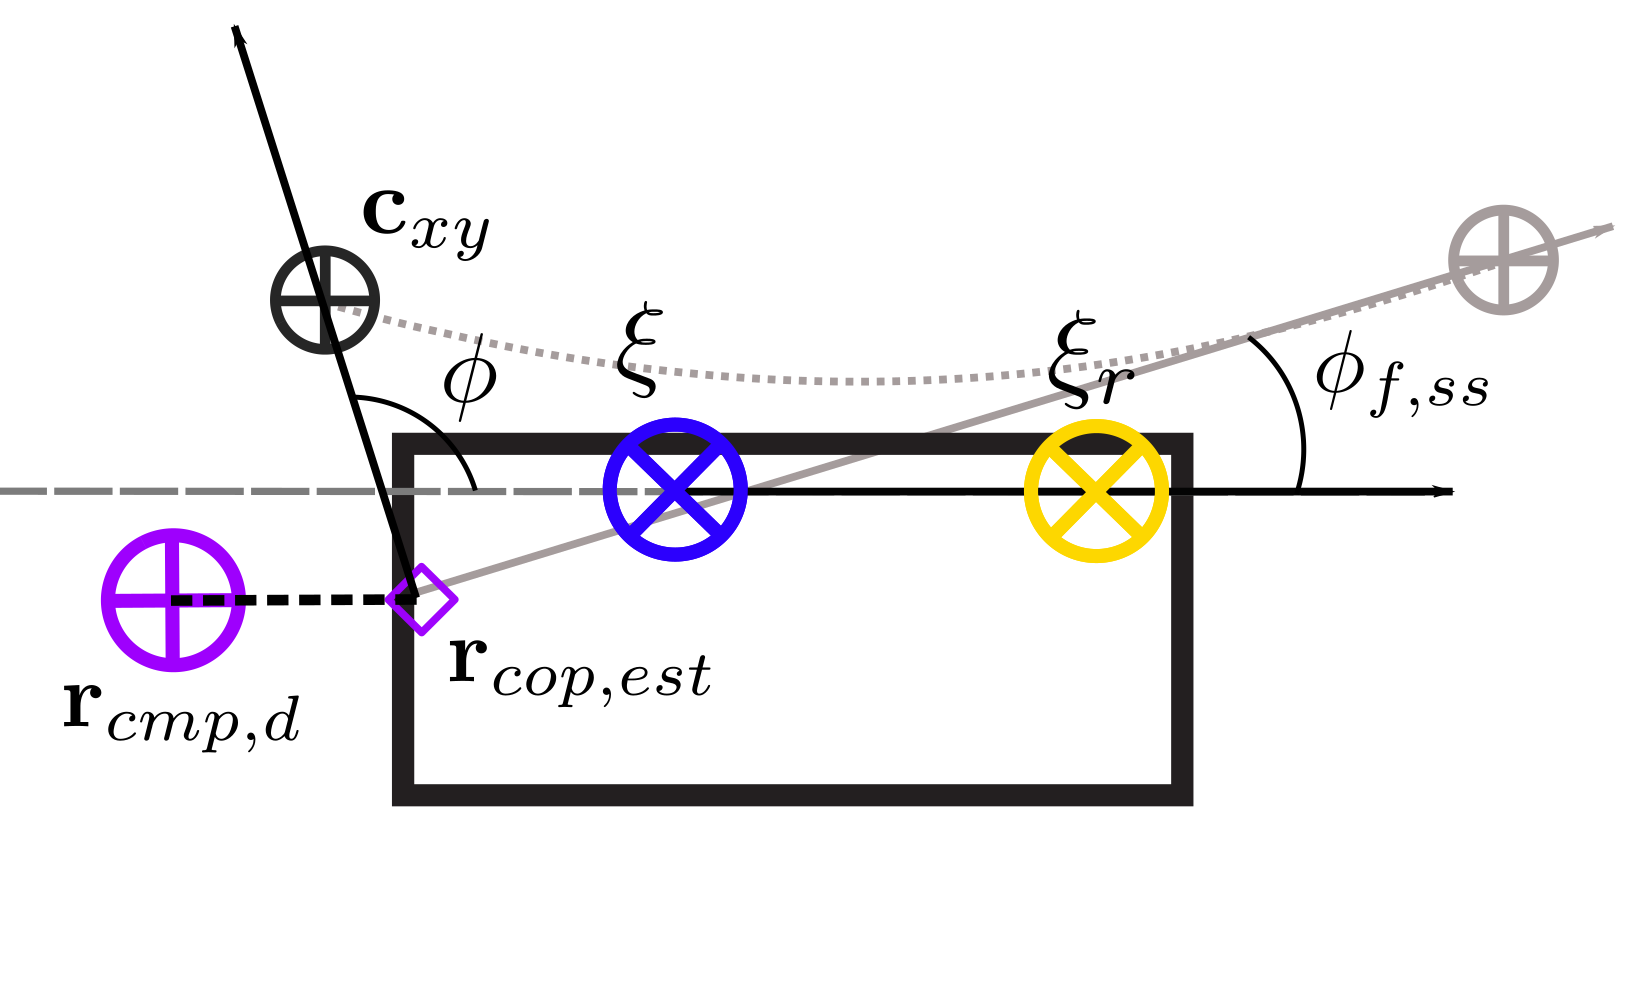
\includegraphics[width=.8\linewidth]{STYLESTUFF/ICPplanStartSSPhiViz.png}
   \caption{}
    \label{fig:phiViza}
  \end{subfigure}
  \begin{subfigure}{0.4\textwidth}
    \centering
  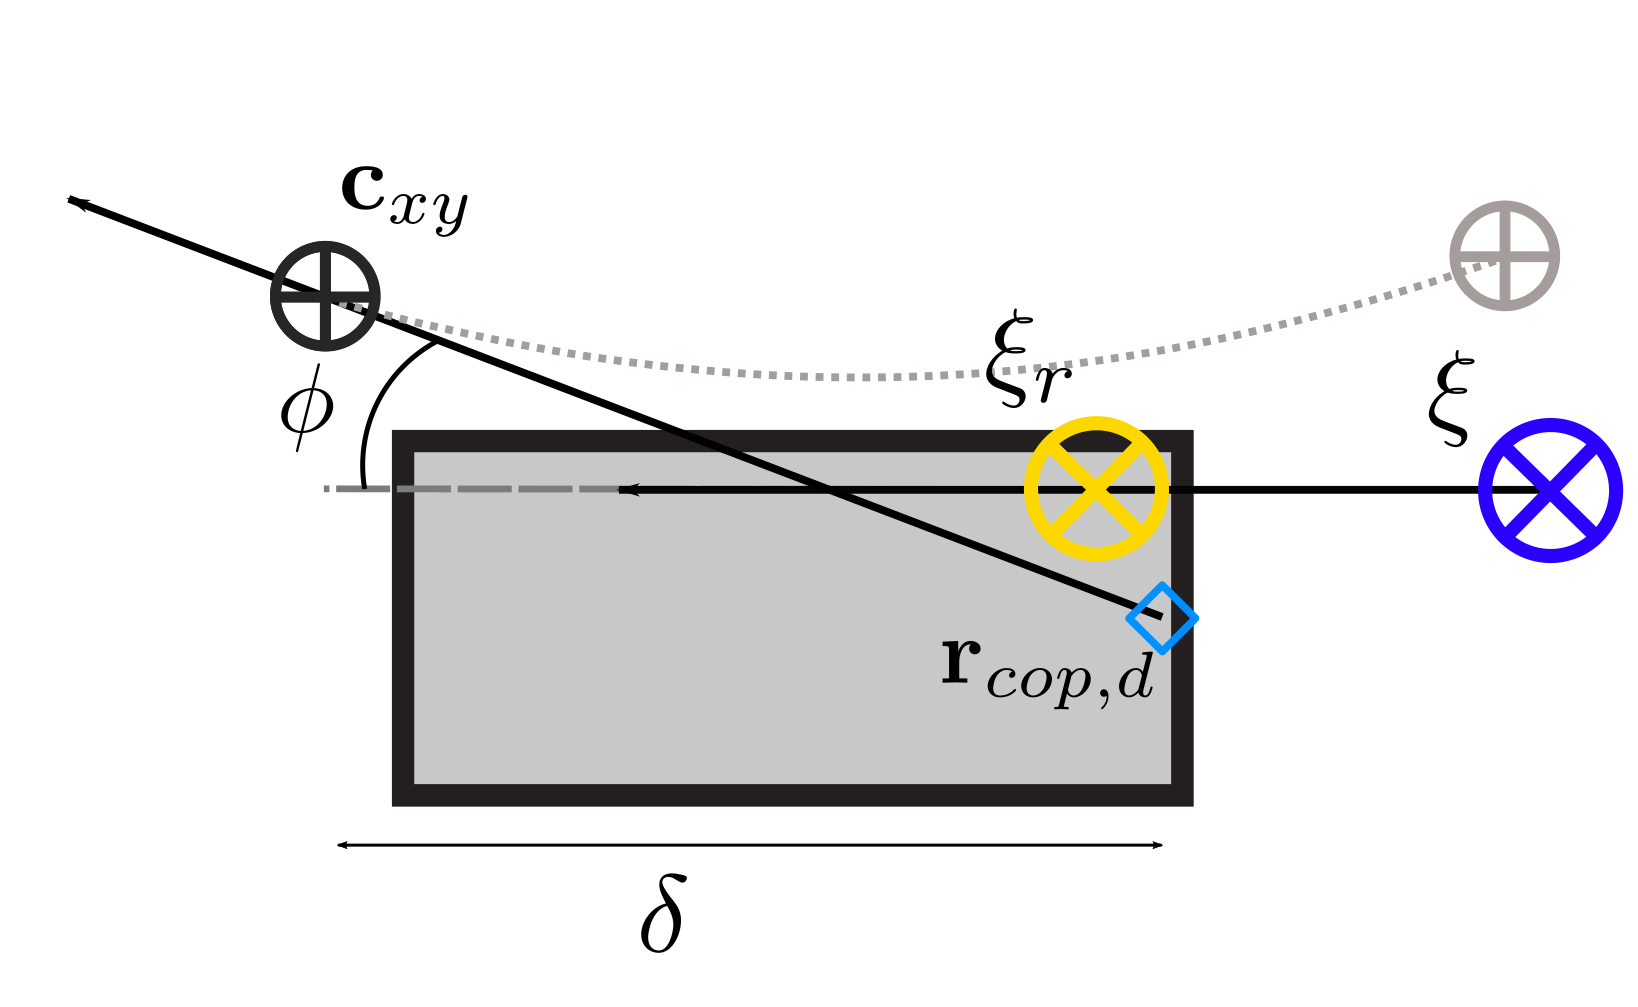
\includegraphics[width=.8\linewidth]{STYLESTUFF/ICPplanStartSSPhiVizNegError.png}
  \caption{}
   \label{fig:phiVizb}
  \end{subfigure}
  \begin{subfigure}{0.4\textwidth}
    \centering
  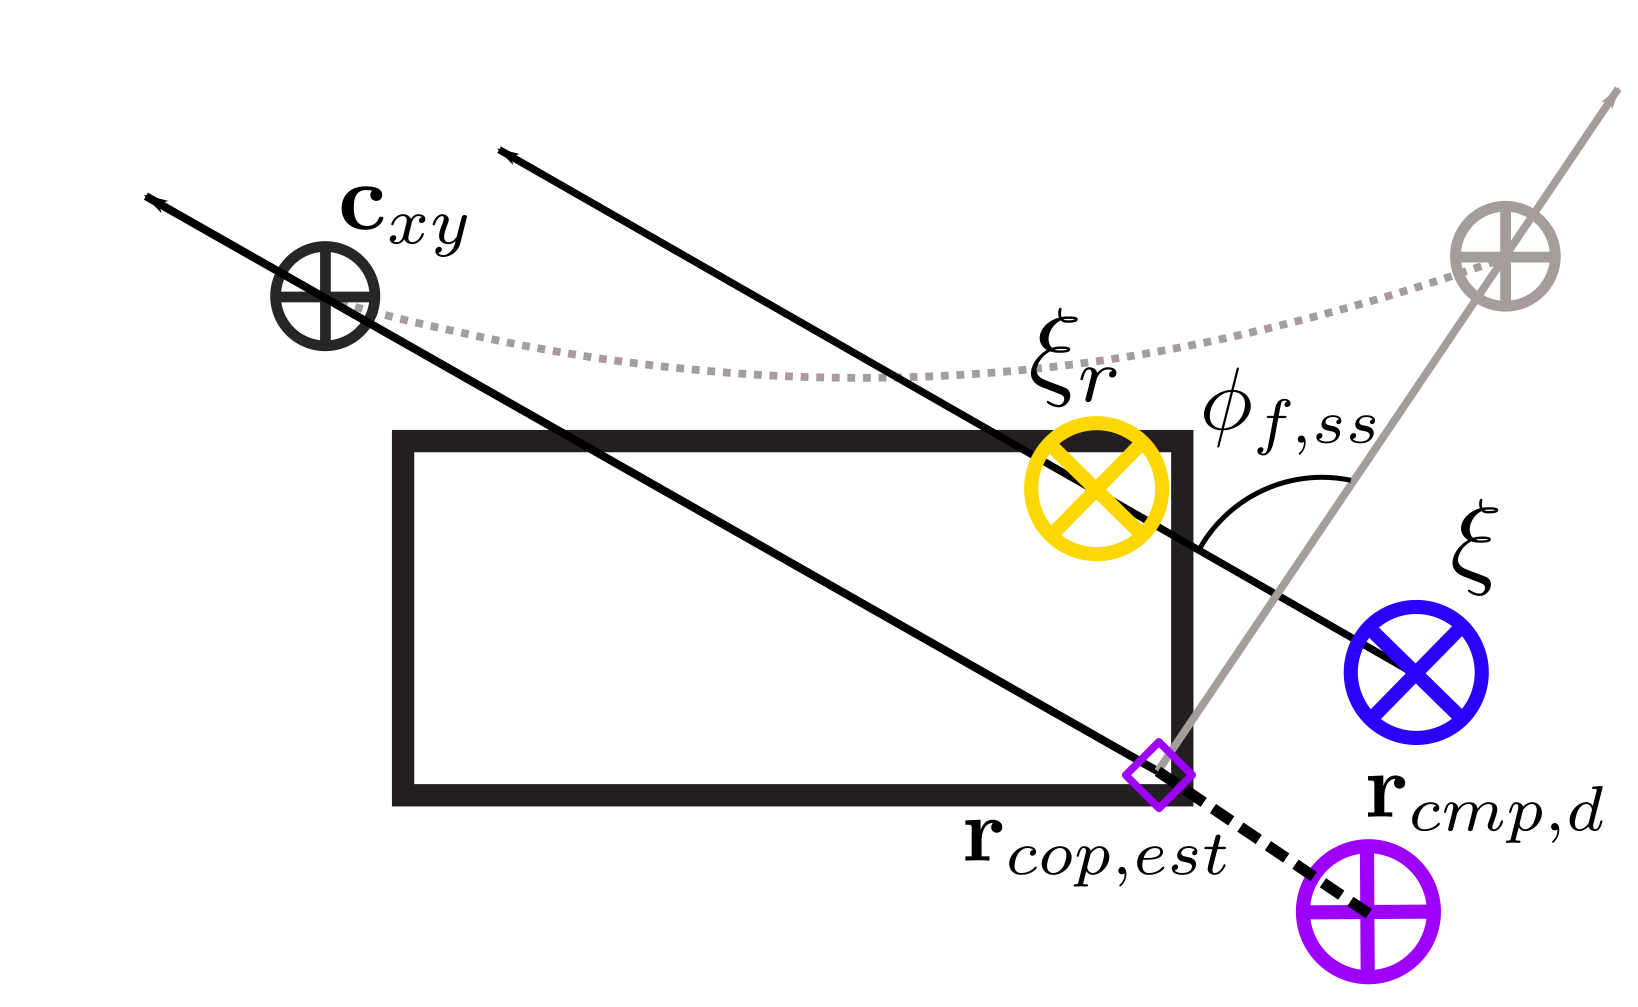
\includegraphics[width=.8\linewidth]{STYLESTUFF/ICPplanStartSSPhiViz0.png}
    \caption{}
     \label{fig:phiVizc}
  \end{subfigure}
  \begin{subfigure}{0.4\textwidth}
    \centering
  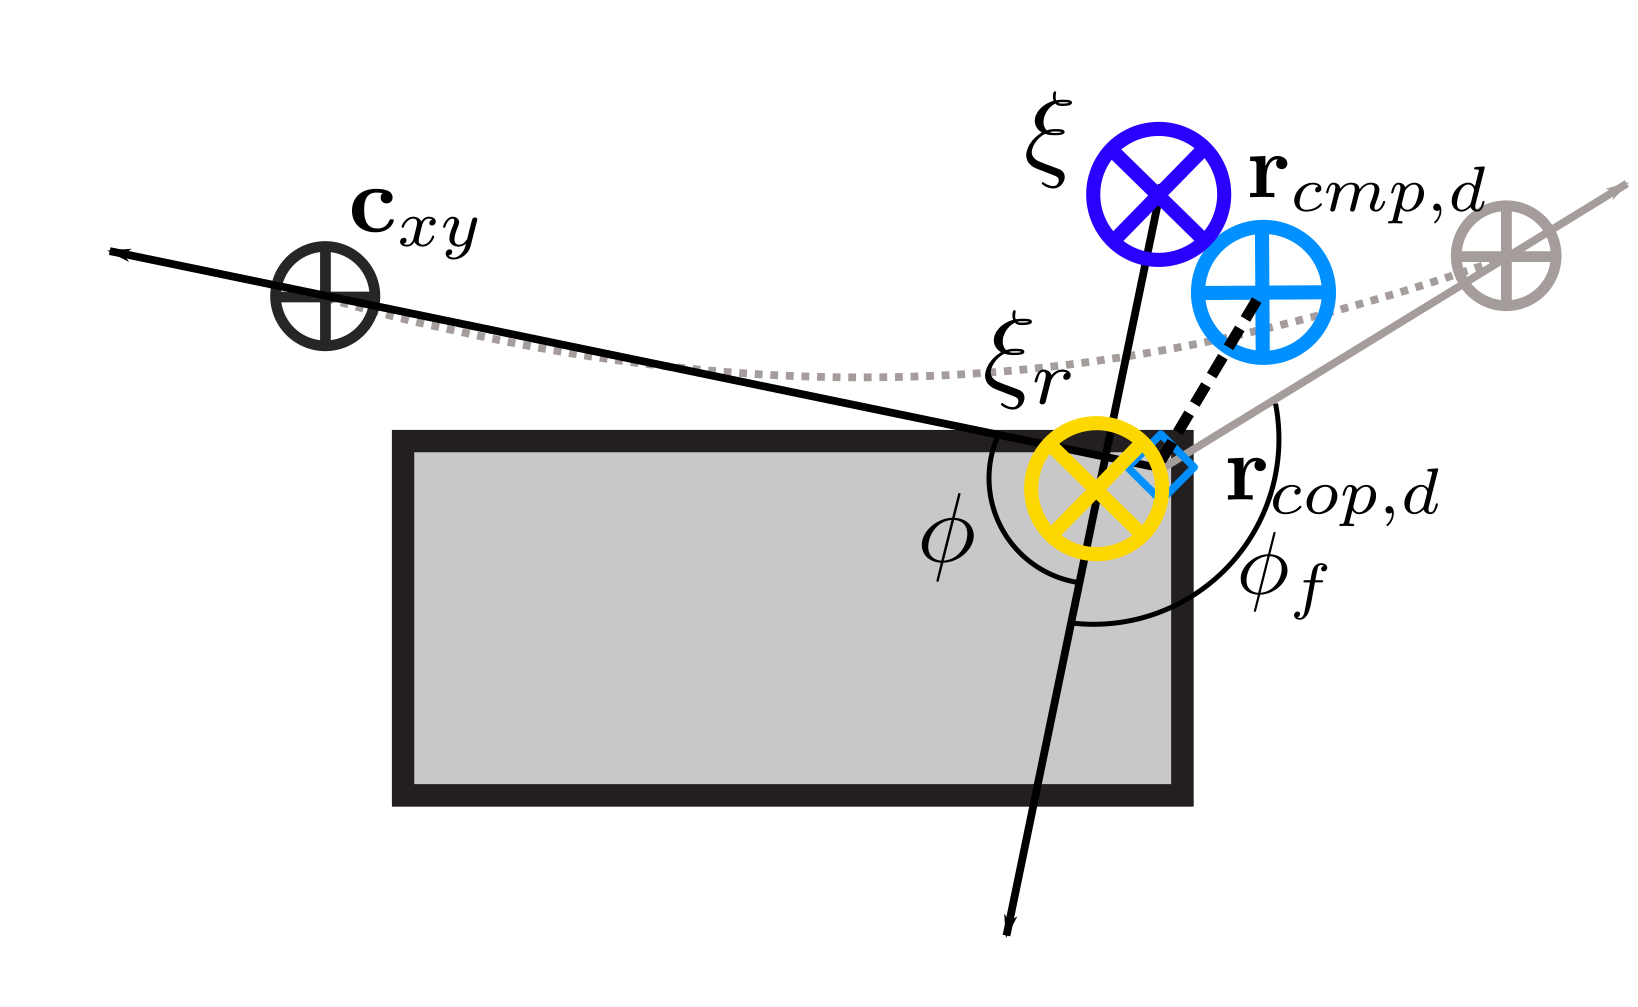
\includegraphics[width=.8\linewidth]{STYLESTUFF/ICPplanStartSSPhiViz90.png}
    \caption{}
     \label{fig:phiVizd}
  \end{subfigure}
    \begin{subfigure}{0.4\textwidth}
    \centering
  \includegraphics[width=.8\linewidth]{STYLESTUFF/ICPplanStartSSPhiVizLeftError.png}
    \caption{}
     \label{fig:phiVize}
  \end{subfigure}
  \begin{subfigure}{0.4\textwidth}
    \centering
  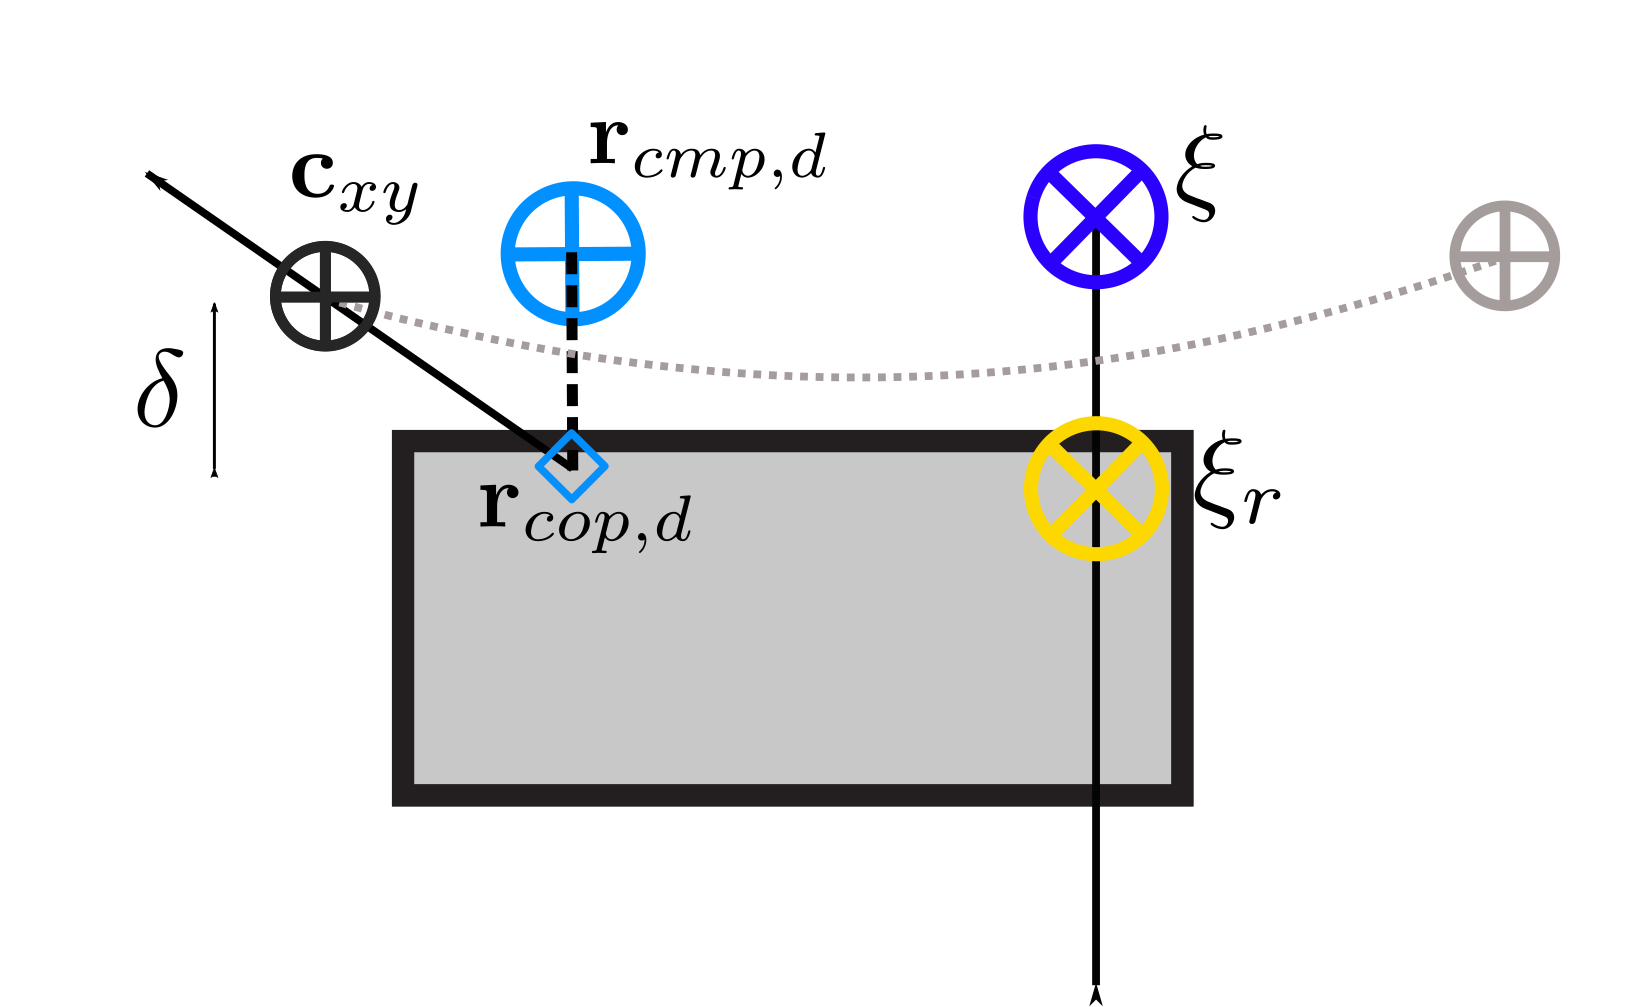
\includegraphics[width=.8\linewidth]{STYLESTUFF/ICPplanStartSSPhiVizRightError.png}
    \caption{}
     \label{fig:phiVizf}
  \end{subfigure}
  \caption{Vizualizations of $\phi$ and $\delta$ for the configuration at start of \ac{SS}. (a) Negative $\icpe$ in sagittal plane, (b) positive $\icpe$ in sagital plane, (c) $\phi=0$, (d) $\delta=0$, (e) case where $\rcmpd$ is expected to move to the front of the foot, (f) the same case, but $\rcmpd$ is on the other side of the polygon.}
  \label{fig:phiViz}
\end{figure}

% Methods
\section{Method}
The goal is to activate the bang-bang control law of the previous chapter in cases where $\delta$ is relatively large and $\phi$ is relatively small or does not play an important role.

During the standing tests in the previous chapter, the needed acceleration was always upward. During walking, the needed vertical acceleration can be downward as well. In the case of a frontal push in the beginning of \ac{SS} for example, the robot needs to speed up the follow the dynamic plan, and thus has to lower its height. The alignment angle $\phi$ and the distance $\delta$ however, are relatively misaligned and small for the frontal push. At the end of \ac{SS}, the distance $\delta_f$ and alignment $\phi_f$ are improved. Therefore, for frontal pushes a phase is considered that \textit{prepares} for a positive `bang' by gradually lowering the robots \ac{CoM} height, instead of applying an instant `bang'.

The following three phases can be selected by the \ac{3D} control law if the $\rcmpd$ touches the polygon edge:
\begin{itemize}
	\item \textbf{Positive alignment}: At the current control tick, $\phi$ is relatively misaligned and $\delta$ relatively large for a push in the sagittal plane, or $\delta$ is relatively large for a push in the coronal plane. Also, $\phi$ has to be smaller than $\frac{1}{2}\pi$ [rad], as the virtual leg must be in direction of the \ac{ICP} error to make additional force effective. A bang-bang action is activated that starts with a positive `bang'.
	\item \textbf{Prepare}: At the current control tick, $\phi$ is relatively misaligned or $\delta$ is relatively small, but $\phi_f$ and $\delta_f$ are at values suitable for the positive alignment phase. The \ac{CoM} height is gradually lowered to the minimum height, after which the `bang-bang' action of the positive alignment phase is activated.
	\item \textbf{Default}: All decisions variables $\phi$, $\delta$, $\phi_f$ and $\delta_f$ are at such values, that vertical \ac{CoM} motion does not improve recovery. The default height control law is used and no additional height changes are considered.
\end{itemize}

For the maximum height constraint $\zmax$, the same parameters as for the standing tests is used in the first half of \ac{SS}. In the second half, the maximum height constraint is linearly interpolated between the maximum height constraint for standing and a maximum height constraint at the end of \ac{SS}.  For the minimum height constraint $\zmin$, a constant value is considered. The height constraints are visually explained in \figref{fig:heightconstraints}.

The prepare phase uses the time it takes to accelerate from the minimum height constraint to the maximum height constraint. This time uses the kinetic and potential energy:
\begin{equation}
	\zmin + \frac{1}{2}\ddzc t_{\zmin \rightarrow \zmax}^2 + \frac{1}{2}\frac{(\ddzc t_{\zmin \rightarrow \zmax})^2}{\ddzalpha \ddzc} = \zmax,
\end{equation}
where $t_{\zmin \rightarrow \zmax}$ is the time from the minimum height constraint to the maximum, considering a zero initial vertical velocity.
This solution for the time reads as:
\begin{equation}
 t_{\zmin \rightarrow \zmax}= \sqrt{\frac{2(\zmax - \zmin)}{\ddzc + \frac{\ddzc}{\ddzalpha} }}.
\end{equation}

This time is used to determine the moment when the first `bang' should be activated. The known remaining time in \ac{SS} $t_{r}$ is shortened by $ t_{\zmin \rightarrow \zmax}$:
\begin{equation}
	t_{z \rightarrow \zmin} =t_{r} - t_{\zmin \rightarrow \zmax},
\end{equation}
where $t_{z \rightarrow \zmin} $ is the time available to move from the current height $z$ to the minimum height $\zmin$. Using this time, at every control tick the desired acceleration $\ddzd$ is computed by using the equation:
\begin{align}
	z + \dot{z}t_{z \rightarrow \zmin} + \frac{1}{2}\ddzd t_{z \rightarrow \zmin}^2 - \frac{1}{2}\frac{(\ddzd t_{z \rightarrow \zmin} + \dot{z})^2}{\ddzalpha \ddzc} &= \zmin, \\
	\underbrace{-\frac{1}{2}\frac{t_{z \rightarrow \zmin}^2}{\ddzalpha \ddzc}}_a \ddzd^2 + \underbrace{(\frac{1}{2}t_{z \rightarrow \zmin}^2-\frac{t_{z \rightarrow \zmin}}{\ddzalpha \ddzc} \dot{z})}_b \ddzd + \underbrace{z -\zmin +\dot{z}t_{z \rightarrow \zmin} -\frac{1}{2}\frac{\dot{z}^2}{\ddzalpha \ddzd}}_c&=0,
\end{align}
which has the solution:
\begin{equation}
 	\ddzd = \frac{-b + \sqrt{b^2-4ac}}{2a}.
\end{equation}
This value for $\ddzd$ is used until $t_{z \rightarrow \zmin}<0$, after which the positive `bang' is activated. 
\begin{figure}[h]
\centering
  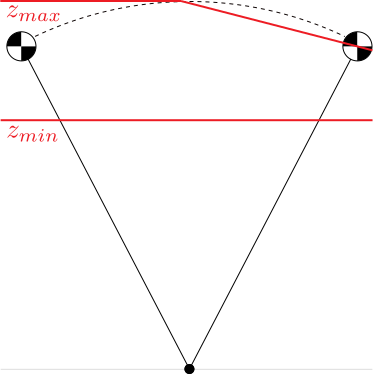
\includegraphics[width=.4\linewidth]{STYLESTUFF/heightconstraints.png}
   \caption{Height constraints through \acf{SS}}
    \label{fig:heightconstraints}
\end{figure} 
% Results
\section{Results}
The following results are obtained by approximating the effects of $\phi$ and $\delta$ by choosing a phase depending on the direction of the \ac{ICP} error with respect to the sagittal direction.
\begin{figure}[h]
\centering
  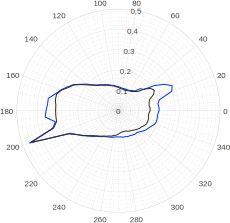
\includegraphics[width=.6\linewidth]{STYLESTUFF/round00.png}
   \caption{Push recovery at the start of \acf{SS}}
    \label{fig:round00}
\end{figure} 
\begin{figure}[h]
\centering
  \includegraphics[width=.6\linewidth]{STYLESTUFF/round02.png}
   \caption{Push recovery at t=$0.2t_{SS}$.}
    \label{fig:round02}
\end{figure} 
\begin{figure}[h]
\centering
  \includegraphics[width=.6\linewidth]{STYLESTUFF/round04.png}
   \caption{Push recovery at t=$0.2t_{SS}$.}
    \label{fig:round04}
\end{figure} 
% Discussion
\section{Discussion}
